\subsubsection{Biological testing\label{sec:bio2}}


Ganguly \textit{et al.} \cite{Ganguly2011} found the MICs of ciprofloxacin and a BHL analogue-ciprofloxacin conjugate \compound{cmpd:SHL4CipMe} under standard planktonic conditions by introducing the compounds to liquid culture. The MICs were found to be ten times lower for ciprofloxacin vs. the conjugate \compound{cmpd:SHL4CipMe} (5 vs 50 um). They then investigated the effect of the compounds on biofilms. The compounds were first cultured at 25um, with PA liquid culture. As expected, the culture failed to grow and form biofilm in the presence of ciprofloxacin, but did grow in the presence of the conjugate \compound{cmpd:SHL4CipMe}. They then cultured biofilm for 24 hours before adding the compounds, and found that, in contrast, the conjugate \compound{cmpd:SHL4CipMe} disrupted the biofilm more effectively than ciprofloxacin. When the biofilm was cultured for 48 or 72 hours the conjugate similarly disruptive effects, whereas ciprofloxacin 'did not show any significant antibacterial activity'.

This work 

All conjugates were tested for growth inhibition (MIC), biofilm formation inhibition and activity against nascent (24 h) and established (48 h) biofilms in \textit{P. aeruginosa} and \textit{S. aureus}.

The conjugates shown in \ref{fgr:finals_1} were tested, as well as BHL \compound{cmpd:HL4}, HHQ \compound{cmpd:HHQ}, PQS \compound{cmpd:PQS}, ciprofloxacin \compound{cmpd:Cip}, methyl ciprofloxacin \compound{cmpd:CipMe}, the alkynyl ciprofloxacin derivative \compound{cmpd:Y4Cip}, the \textit{tert}-butyl ester ciprofloxacin derivative \compound{cmpd:tBuOO4CipMe}, the carboxylic acid ciprofloxacin derivative \compound{cmpd:HOO4CipMeTFA}, trimethoprim \compound{cmpd:Tri} and the alkynyl trimethoprim derivative \compound{cmpd:Y4Tri}.

Cultures were grown in the presence of the compounds at a range of 6 concentrations from 25 to 0.125 $\mu$M. MICs were calculated by fitting a modified Gompertz function\cite{Lambert2016}. An example of the fitting is shown in \ref{fgr:Gompertz}. 

\begin{figure}[H]
	\begin{center}
		\schemeref[HL2T4Cip]{cmpd:HL2T4Cip}
		\schemeref[HL4T4Cip]{cmpd:HL4T4Cip}
		\schemeref[HL6T4Cip]{cmpd:HL6T4Cip}
		\schemeref[6HHQT4Cip]{cmpd:6HHQT4Cip}
		\schemeref[HL4T4Tri]{cmpd:HL4T4Tri}
		\schemeref[HL6T4Tri]{cmpd:HL6T4Tri}
		\schemeref[6HHQT4Tri]{cmpd:6HHQT4Tri}
		\schemeref[PQST4Tri]{cmpd:PQST4Tri}		\schemeref[SHL4CipMe]{cmpd:SHL4CipMe}
		\schemeref[SHL4T4Cip]{cmpd:SHL4T4Cip}
		\schemeref[SHL4THCip]{cmpd:SHL4THCip}
		\schemeref[SHL4TMeCip]{cmpd:SHL4TMeCip}
		\schemeref[2MeOA4CipMe]{cmpd:2MeOA4CipMe}
		\schemeref[3MeOA4CipMe]{cmpd:3MeOA4CipMe}
		\schemeref[2MeOA4T4Cip]{cmpd:2MeOA4T4Cip}
		\schemeref[3MeOA4T4Cip]{cmpd:3MeOA4T4Cip}
		\schemeref[HOcy5NH4CipMe_RR]{cmpd:HOcy5NH4CipMe_RR}
		\schemeref[HOcy5NH4CipMe_SS]{cmpd:HOcy5NH4CipMe_SS}
		\schemeref[Ocy5NH4CipMe_S]{cmpd:Ocy5NH4CipMe_S}
		\schemeref[HOcy5NH4T4Cip_RR]{cmpd:HOcy5NH4T4Cip_RR}
		\schemeref[HOcy5NH4T4Cip_SS]{cmpd:HOcy5NH4T4Cip_SS}
		\schemeref[HOcy6NH4CipMe]{cmpd:HOcy6NH4CipMe}
		\schemeref[Ocy6NH4CipMe]{cmpd:Ocy6NH4CipMe}
		\schemeref[HOcy6NH4T4Cip]{cmpd:HOcy6NH4T4Cip}
		\schemeref[Ocy6NH4T4Cip]{cmpd:Ocy6NH4T4Cip}
		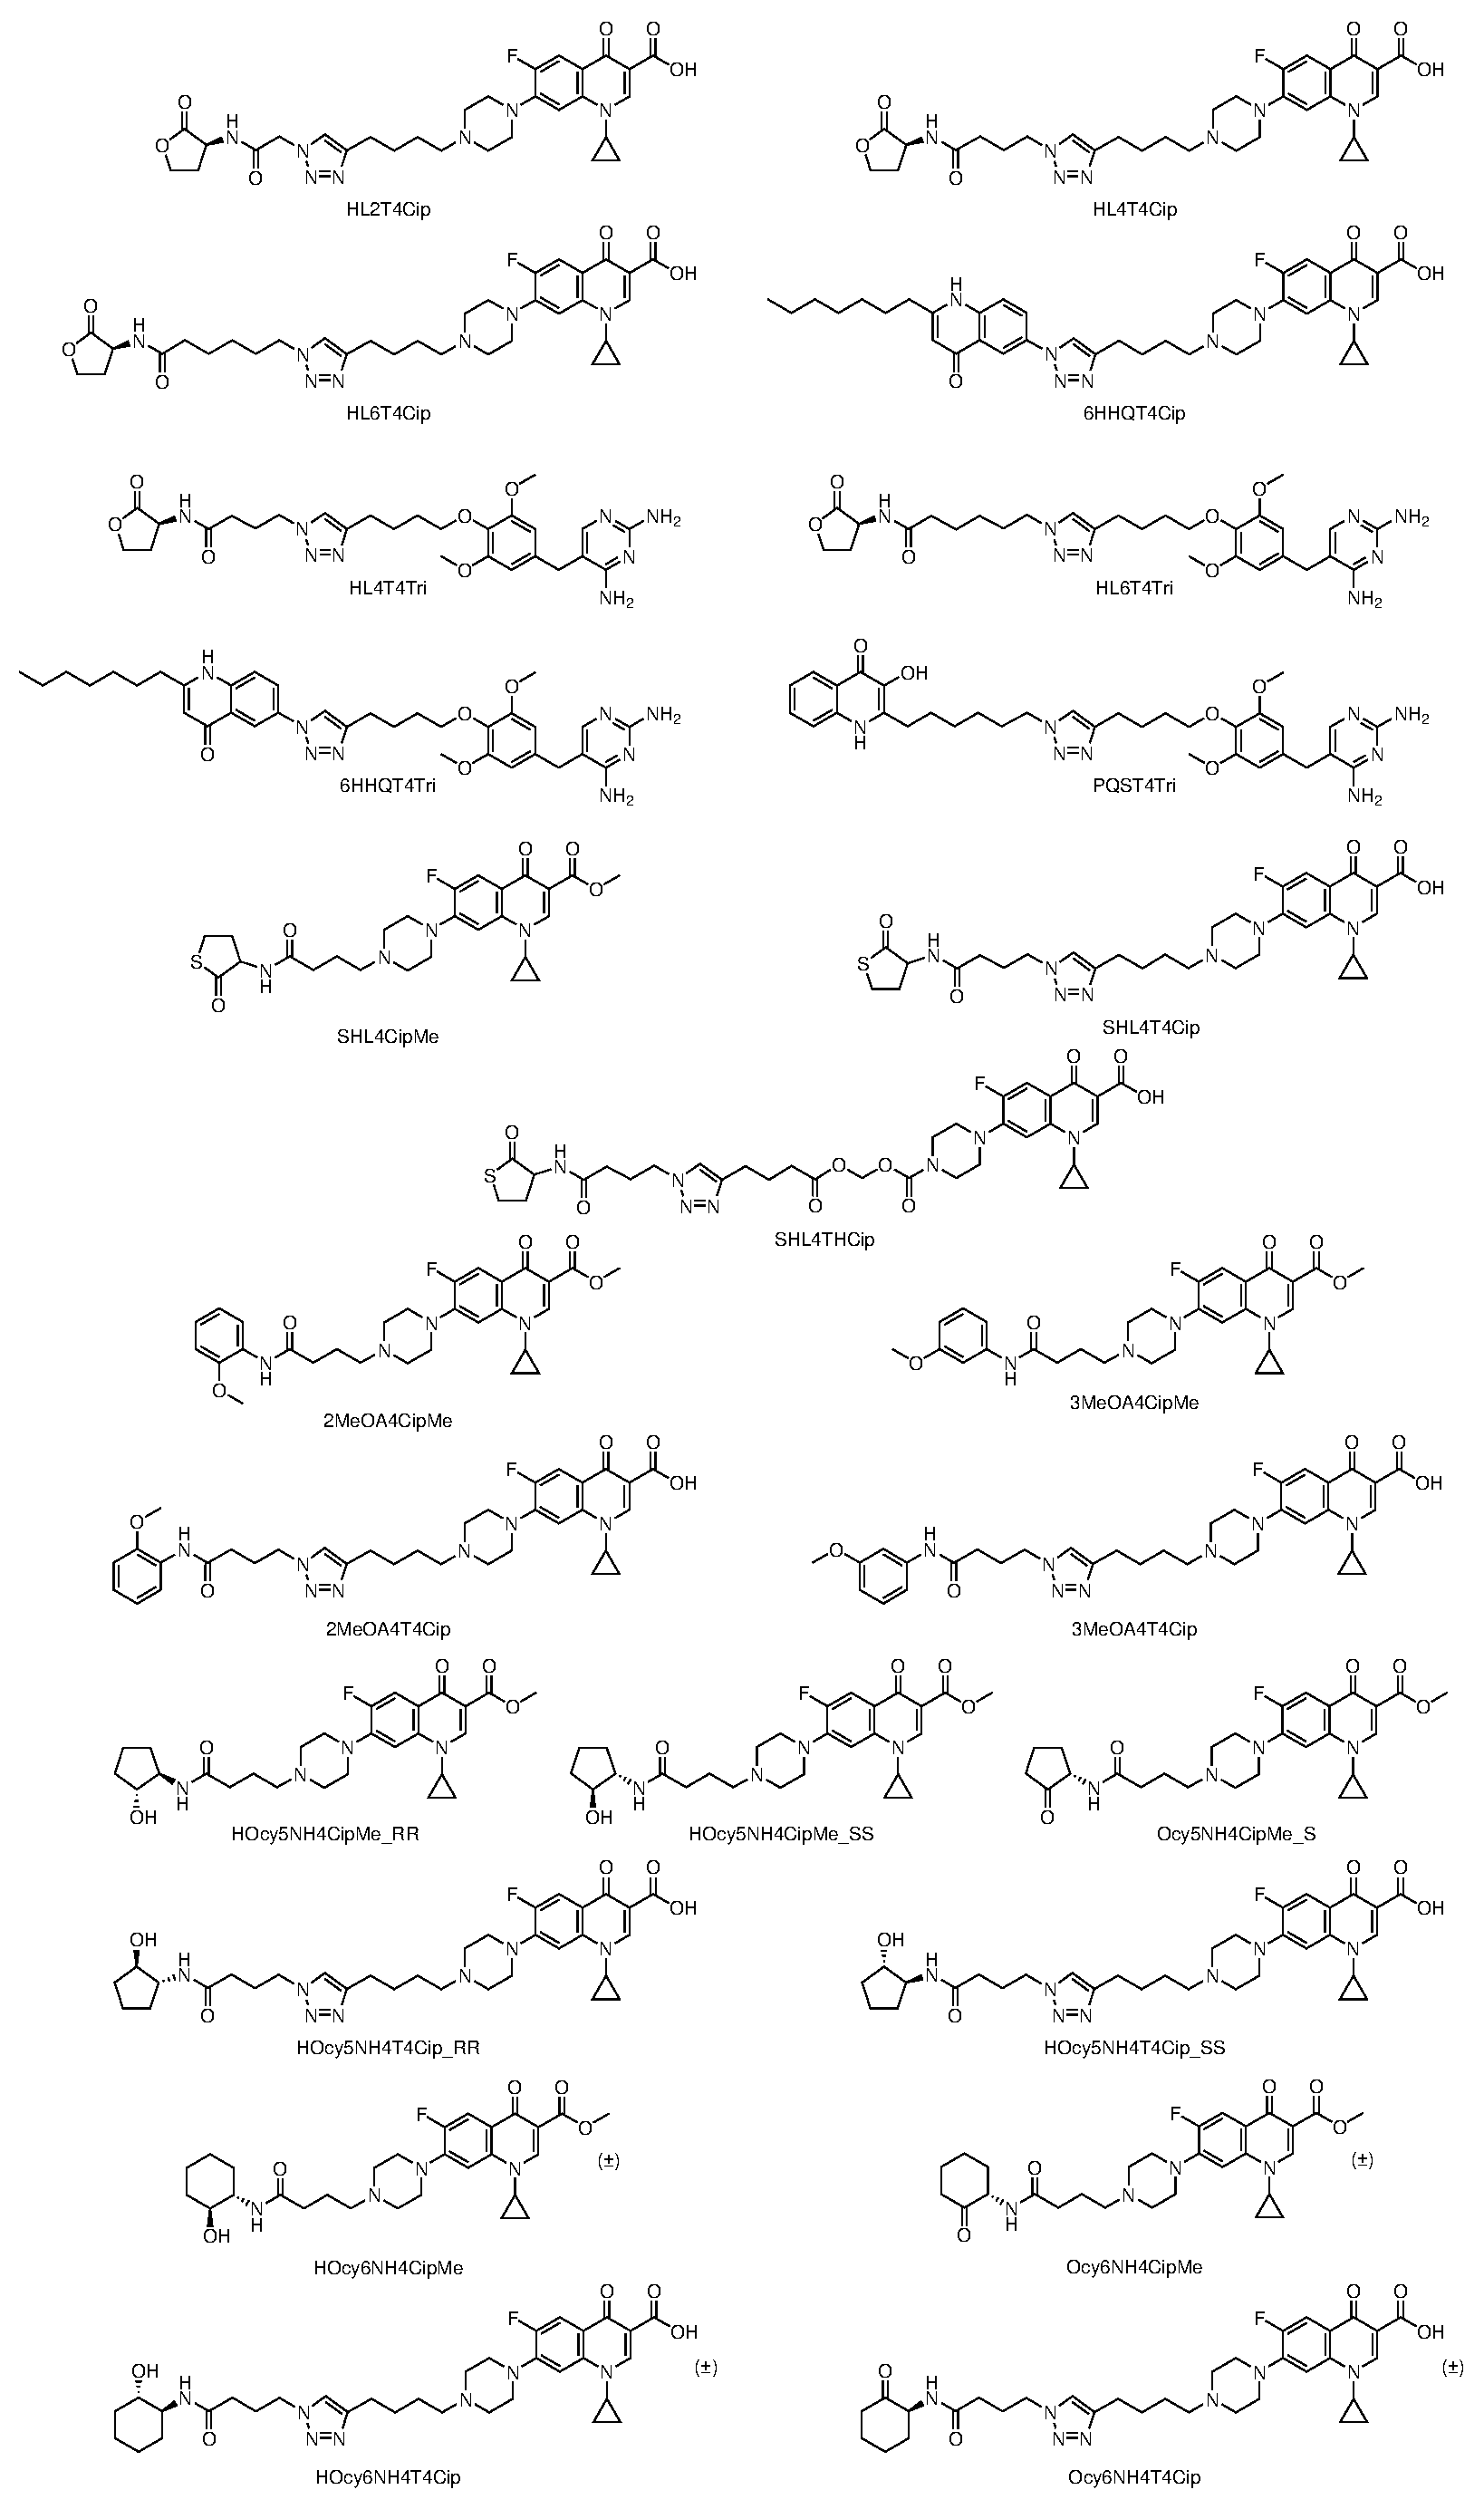
\includegraphics[scale=0.5]{finals_1}
		\caption{
 		\label{fgr:finals_1}}
	\end{center}
\end{figure}

\subsection{Determination of MICs}

The Minimum Inhibitory Concentration (MIC) is defined as the lowest concentration of an antimicrobial ingredient or agent that is bacteriostatic (prevents the visible growth of bacteria). MICs are used to evaluate the antimicrobial efficacy of various compounds by measuring the effect of decreasing concentrations of antibiotic/antiseptic over a defined period in terms of inhibition of microbial population growth.  

\subsubsection{PAO1}

Bar Graphs
MIC 8h for all HSL analogue conjugates (9-25 and controls)
"24h
"48h

Growth curves for interesting ones at lowest conc compare to controls?
10,11,12,15,16,20,21,24,25 (13,14 weird)
Best 11,16,20

\subsubsection{YM64}

Bar Graphs
MIC 8h for all HSL analogue conjugates (9-25 and controls)
"24h
"48h

Growth curves for interesting ones at lowest conc compare to controls?
(can't see 9-16 graphs, check)
9,10,11,12,15,16
17-21,24,25
Best 10,11,12,15,16,20,21,24,25

\subsubsection{HGS4}
(can't see 9-16 graphs, check)
1-25 no inhibition
except 11 a bit


\subsubsection{HGS4 complemented}

11,16,19,20,21,22,24,25

\subsection{Determination of anti-biofilm activity}

Biofilm growth was measured using crystal violet staining\cite{OToole1998}.

\subsubsection{Effect on biofilm formation}





\subsubsection{Biofilm disruption}



Biofilms can drastically increase MIC for many antibiotics \cite{Ceri1999}. For ciprofloxacin in \textit{P. aeruginosa} the MIC increases by 16 fold. 

Ganguly \textit{et al.} \cite{Ganguly2011} found the MICs of ciprofloxacin and a BHL analogue-ciprofloxacin \compound{cmpd:SHL4CipMe} conjugate under standard planktonic conditions by introducing the compounds to liquid culture. The MICs were found to be ten times lower for ciprofloxacin vs. the conjugate \compound{cmpd:SHL4CipMe} (5 vs 50 um). They then investigated the effect of the compounds on biofilms. The compounds were first cultured at 25um, with PA liquid culture. As expected, the culture failed to grow and form biofilm in the presence of ciprofloxacin, but did grow in the presence of the conjugate \compound{cmpd:SHL4CipMe}. They then cultured biofilm for 24 hours before adding the compounds, and found that, in contrast, the conjugate \compound{cmpd:SHL4CipMe} disrupted the biofilm more effectively than ciprofloxacin. When the biofilm was cultured for 48 or 72 hours the conjugate similarly disruptive effects, whereas ciprofloxacin 'did not show any significant antibacterial activity'.

Ganguly \textit{et al.} used Bac-Light Live/Dead staining and confocal microscopy to image the biofilms, whereas so far I have used crystal violet staining. Crystal violet does not differentiate between live or dead cells, and so might not pick up on the antibacterial effects of compounds. However, their confocal microscopy results show a quantifiable decrease in biofilm thickness, and it may be possible to detect this using crystal violet.

The conjugate \compound{cmpd:SHL4CipMe} developed by Ganguly \textit{et al.} contained a thiolactone AHL. The unconjugated thiolactone BHL \compound{cmpd:SHL4} was shown to have 'either enhanced uptake or functional activity' when compared with BHL \compound{cmpd:HL4}. Therefore it seems possible that my compounds may not show enhanced antibiotic activity, where thiolactone analogues might.